%% Teaser (two columns). Graphic: figures/teaser.png
\begin{figure*}[t]
  \centering
  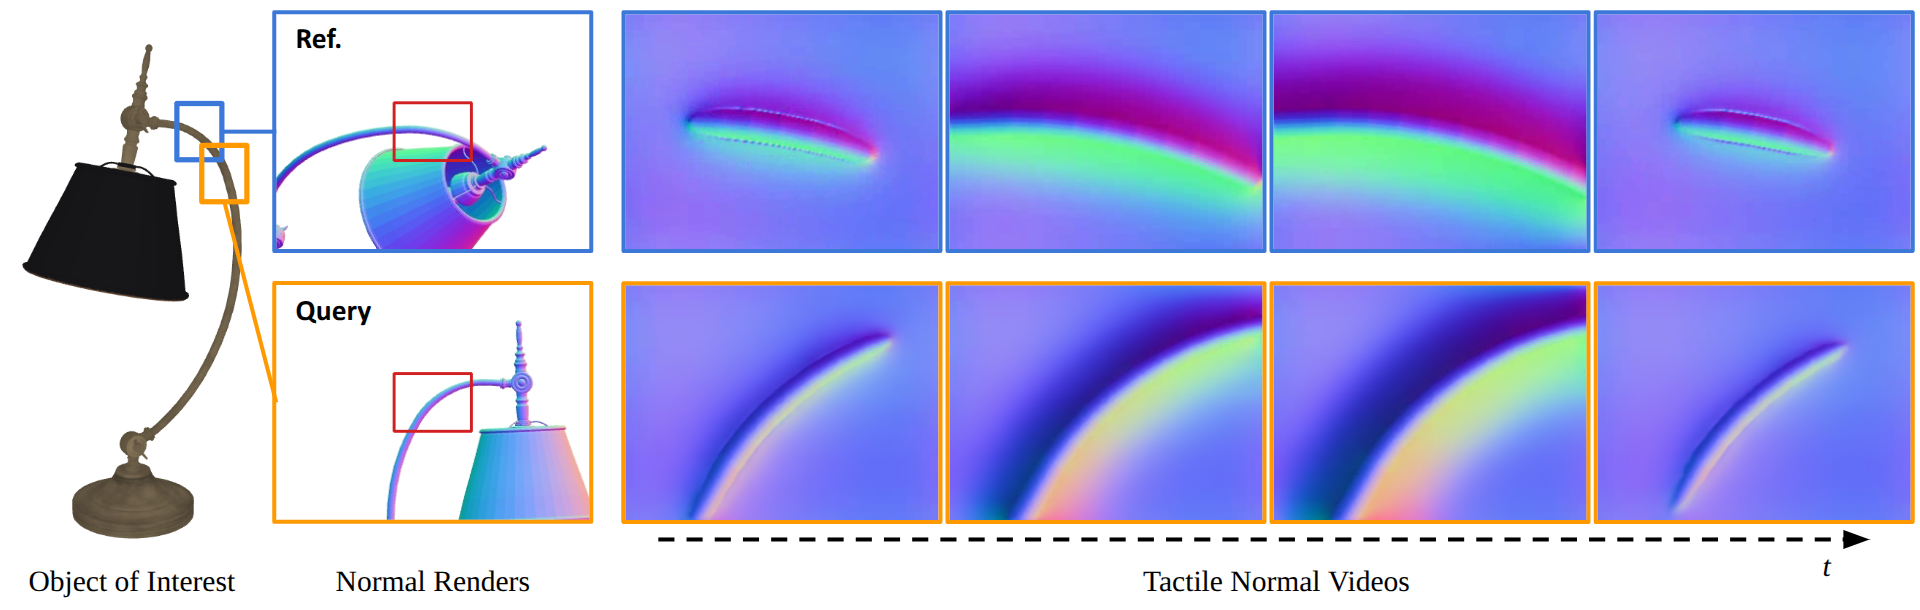
\includegraphics[width=\linewidth]{figures/teaser.png}
  \caption{\textbf{Tactile analogies.} Left: the object, with a reference touch boxed in blue and a
    new, untouched query location in orange. Middle: the normal render at each sensor pose, covering
    four times the sensor footprint, with the red box marking the sensor's own patch. Right: the
    tactile normal videos, four frames of a press that pushes in and withdraws, time running left to
    right. Given the reference touch and the geometry at both locations, our method predicts the
    video the sensor would measure at the query location (bottom right).}
  \label{fig:teaser}
\end{figure*}
